\section{Implementation of the new features}
\nomenclature{ASCII}{American Standard Code for Information Interchange -- a character encoding standard}
\nomenclature{TLSH}{Trend Micro Locality Sensitive Hash}
\nomenclature{HTML}{Hypertext Markup Language}
\nomenclature{XML}{Extensible Markup Language}
\nomenclature{URI}{Uniform Resource Identifier}
\nomenclature{XZ}{lossless data compression program and file format}
\nomenclature{EXIF}{Exchangeable Image File Format}

\subsection[Order-like difference]{Order-like difference}
\nopagebreak[4]{

  Of all the categorized issues, there are several that are identified by a different ordering in the two files. To easily identify these issues,
  ability to mark the files that are different only in the ordering of lines was needed.
  
The solution was to modify comparison of text files, adding the following algorithm of detecting order-like difference:
    \begin{itemize}[noitemsep]
    \item Get the list of lines in the first file that are different from the second file and list of lines from the second file that are different from the first file.
    \item Compare the number of lines in both lists. If they are different, it can be concluded that the difference is not just in ordering of lines. 
    \item If the number of lines is the same, sort them and compare the results element-wise. If that comparison revealed no difference, then the original difference was only in ordering of lines.
    \end{itemize}

The new feature is limited to the plain text and some other file types that are treated as plain text (e.g. HTML, XML).
It was decided there are no sufficient 
use cases to justify the wider range of supported formats.\\\\

Figure \ref{fig:order} shows how the HTML output looks like when run over two HTML files that are different only in the ordering of lines. Note the ``ordering differences only'' line on the top of the section.
\FloatBarrier

\begin{figure}
\centering
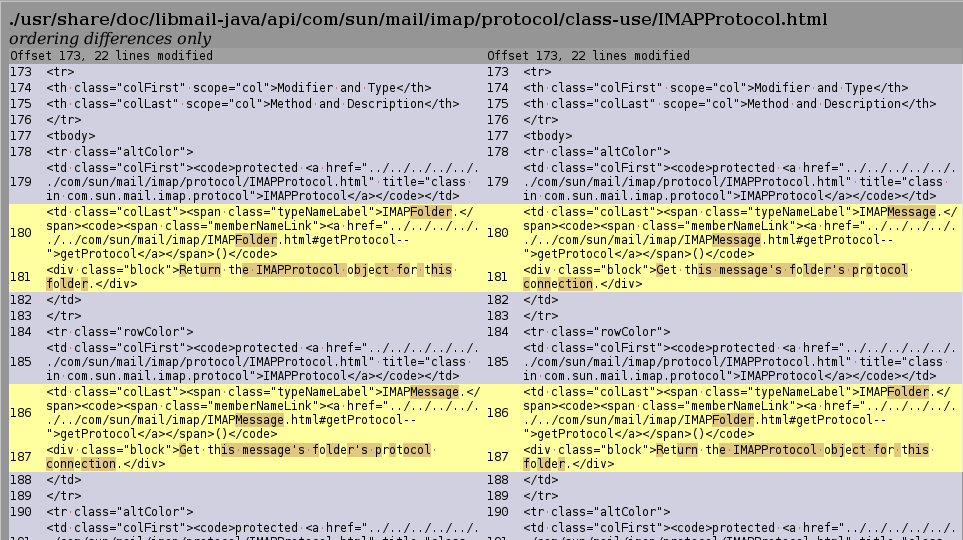
\includegraphics[width=0.95\textwidth]{fig/order-like-diff.png}
\caption{\label{fig:order}Comparison of two HTML files with ordering-only differences.}
\end{figure}

}
\subsection[Improved support for APK files]{Improved support for APK files}
\nopagebreak[4]{
Diffoscope compares APK files using \texttt{apktool}. This tool tries to disassemble the package back to
the project and resource files. The disassembled files are then compared using the suitable tool.

There was a number of improvements made for APK files comparison.
\begin{itemize}[noitemsep]
\item APK metadata, generated by \texttt{apktool} and written into the special file \path{apktool.yml}, is now handled separately from the rest of the files. 
It is renamed into ``APK metadata'' to reflect its contents; in addition, the APK file name itself is removed from the metadata, since the goal of diffoscope is to compare the contents of the file, regardless of their name.
\item APK files difference now includes information about APK file as archive: level of compression, access rights etc. 
This is done using \texttt{zipinfo}, since APK files are essentially a kind of ZIP archive files.
\item \path{AndroidManifest.xml}, a mandatory file for every Android package including the general 
information about it, has a better support now. Previously, these files were compared twice: once in their encoded form and once in the decoded plain text form generated by \texttt{apktool}. Now diffoscope tries to find the difference in the decoded \path{AndroidManifest.xml}, and falls back to the comparison of encoded ones only if the former approach does not reveal any differences.
\end{itemize}

Figure \ref{fig:apk} shows how the HTML output looks like when run over two APK files. The diffoscope version in use has the described features included.
\FloatBarrier

\begin{figure}
\centering
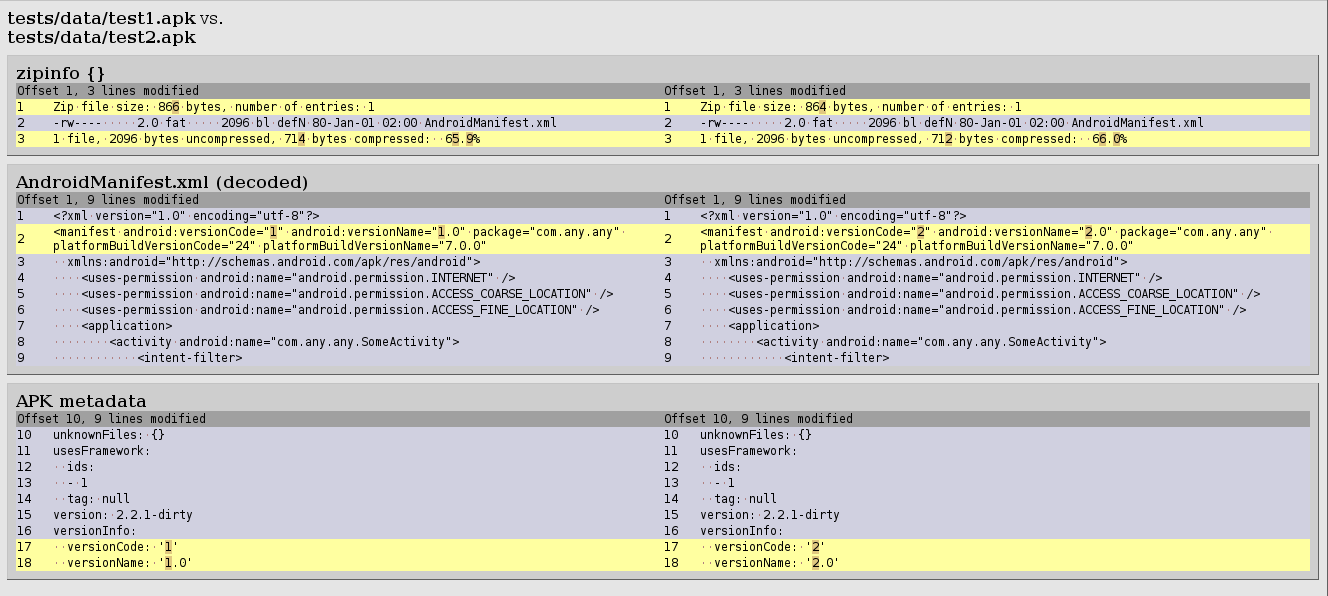
\includegraphics[width=0.95\textwidth]{fig/apk.png}
\caption{\label{fig:apk}Comparison of two APK files.}
\end{figure}

These changes are mostly useful for the F-Droid project \autocite{fdroid}, aiming to provide a collection of free Android applications. As part of the F-Droid project, the F-Droid Verification Server \autocite{fdroid-vfs} was set up, with all the applications being tested for reproducibility automatically.
Better support for APK files allows for a more informative diffoscope output provided for the application that fail these tests.


}
\subsection[Improved support for image files]{Improved support for image files}
\nopagebreak[4]{
Since diffoscope is mainly used to compare packages, support for the images is needed mainly for resource files used in some software. Currently, supported formats include JPEG, ICO, GIF and PNG.

The main approach to comparison of images at the moment involves converting them into ASCII-pseudographics using \texttt{libcaca} and comparing the resulting text. That approach allows for identifying issues related to content of the image, but some information -- such as palette, EXIF data, number of colors -- might be lost. Considering this, the new feature, comparison of image metadata, was added to diffoscope.\\
Metadata comparison is enabled for JPEG and ICO images. Information about the image is retrieved using \texttt{ImageMagick} tool.
The list of image properties extracted include image format, file size, height, width, orientation, compression type, compression quality, colorspace, number of channels and others. Information is extracted in text form and then compared using text comparison.

In addition, in cases where diffoscope is producing HTML output, it is possible to output images without converting them to text form. In these cases, generating ``visual difference'', image, showing the difference in the visual form, can result in a more informative output then pseudographics allows.
This behaviour was implemented in form of providing an additional field for the \texttt{Difference} objects, containing the visual difference images. These images are converted to \texttt{base64} form and embedded into the resulting HTML page using data URI protocol. Two types of visual difference are being generated for each pair of images at the moment:
\begin{itemize}[noitemsep]
  \item Pixel difference -- generated using \texttt{ImageMagick} \texttt{compare} tool. This kind of images underlines all the pixels that have different values for the compared images. This often includes differences which are not normally noticeable by human eye, such as compression artifacts.
  \item Flicker difference -- animation composed by alternating between the two images. Flicker difference is designed to provide a more human-perceptible way to view the difference, as it allows to notice the more significant changes between the two frames. 
\end{itemize}

Currently, the visual difference is computed only for the images of the same size and with only one frame per image, meaning this feature does not support comparing animated GIFs.
}

\subsection[Cross-container comparison]{Cross-container comparison}
\nopagebreak[4]{
The problem of comparing different types of archives was considered to be best solved by alerting fuzzy-matching module.
Diffoscope uses TLSH \autocite{oliver2013tlsh} library that implements fuzzy-matching using special hash values for files. 
By comparing hash values for different files, diffoscope is able to correctly recognize renamed files even when there is difference in the contents.\\\\
However, implementing the similar behaviour for containers was not a trivial task. 
If the container is considered a regular file and the hash is computed as for any other type of file, the result will be dependent on the type of the container, compression method, etc. Another option would be to compute the hash as combination of individual files' hashes. Unfortunately, that approach leads to unnecessary increase in computation time, since every container has to be extracted before finding the correspondence.\\\\
Even more important is the problem of comparing the nested containers. The most common use case is comparing compressed tarballs, e.g. \texttt{TAR.GZ} with \texttt{ZIP} archives. Both approaches described above would fail at this example, since not only the archive type, but the nesting level is different. However, both methods are quite common for software distribution, and it is desirable to have diffoscope compare their content, instead of stopping on the difference in the container type.\\\\
The proposed changes implement the following behaviour:
\begin{itemize}[noitemsep]
\item If both compared objects are containers, but have different types, they are compared by finding difference in:
\begin{itemize}[noitemsep]
\item Type of container
\item List of contents
\item Content
\end{itemize}
\item If one of the compared containers has one of following types: \texttt{gzip}, \texttt{bzip2}, \texttt{xz}, \texttt{dex}, it gets unpacked and the contents are compared. This can be safely done because all of these container types are guaranteed to have only one member. This way, the most common use case of nested containers is addressed.
\end{itemize}

The described changes for cross-container comparison are currently under review and therefore are not included in diffoscope yet.
}

%\cleardoublepage
